%%%%%%%%%%%%%%%%%%%%%%%%%%%%%%%%%%%%%%%%%
% Lachaise Assignment
% LaTeX Template
% Version 1.0 (26/6/2018)
%
% This template originates from:
% http://www.LaTeXTemplates.com
%
% Authors:
% Marion Lachaise & François Févotte
% Vel (vel@LaTeXTemplates.com)
%
% License:
% CC BY-NC-SA 3.0 (http://creativecommons.org/licenses/by-nc-sa/3.0/)
% 
%%%%%%%%%%%%%%%%%%%%%%%%%%%%%%%%%%%%%%%%%

%----------------------------------------------------------------------------------------
%	PACKAGES AND OTHER DOCUMENT CONFIGURATIONS
%----------------------------------------------------------------------------------------

\documentclass{article}

%%%%%%%%%%%%%%%%%%%%%%%%%%%%%%%%%%%%%%%%%
% Lachaise Assignment
% Structure Specification File
% Version 1.0 (26/6/2018)
%
% This template originates from:
% http://www.LaTeXTemplates.com
%
% Authors:
% Marion Lachaise & François Févotte
% Vel (vel@LaTeXTemplates.com)
%
% License:
% CC BY-NC-SA 3.0 (http://creativecommons.org/licenses/by-nc-sa/3.0/)
% 
%%%%%%%%%%%%%%%%%%%%%%%%%%%%%%%%%%%%%%%%%

%----------------------------------------------------------------------------------------
%	PACKAGES AND OTHER DOCUMENT CONFIGURATIONS
%----------------------------------------------------------------------------------------

\usepackage{amsmath,amsfonts,stmaryrd,amssymb} % Math packages

\usepackage{enumerate} % Custom item numbers for enumerations

\usepackage[ruled]{algorithm2e} % Algorithms

\usepackage[framemethod=tikz]{mdframed} % Allows defining custom boxed/framed environments

\usepackage{listings} % File listings, with syntax highlighting
\lstset{
	basicstyle=\ttfamily, % Typeset listings in monospace font
}

\usepackage[hidelinks,colorlinks=true]{hyperref}

%----------------------------------------------------------------------------------------
%	DOCUMENT MARGINS
%----------------------------------------------------------------------------------------

\usepackage{geometry} % Required for adjusting page dimensions and margins

\geometry{
	paper=a4paper, % Paper size, change to letterpaper for US letter size
	top=2.5cm, % Top margin
	bottom=3cm, % Bottom margin
	left=2.5cm, % Left margin
	right=2.5cm, % Right margin
	headheight=14pt, % Header height
	footskip=1.5cm, % Space from the bottom margin to the baseline of the footer
	headsep=1.2cm, % Space from the top margin to the baseline of the header
	%showframe, % Uncomment to show how the type block is set on the page
}

%----------------------------------------------------------------------------------------
%	FONTS
%----------------------------------------------------------------------------------------

\usepackage[utf8]{inputenc} % Required for inputting international characters
\usepackage[T1]{fontenc} % Output font encoding for international characters

%\usepackage{XCharter} % Use the XCharter fonts

%----------------------------------------------------------------------------------------
%	COMMAND LINE ENVIRONMENT
%----------------------------------------------------------------------------------------

% Usage:
% \begin{commandline}
%	\begin{verbatim}
%		$ ls
%		
%		Applications	Desktop	...
%	\end{verbatim}
% \end{commandline}

\mdfdefinestyle{commandline}{
	leftmargin=10pt,
	rightmargin=10pt,
	innerleftmargin=15pt,
	middlelinecolor=black!50!white,
	middlelinewidth=2pt,
	frametitlerule=false,
	backgroundcolor=black!5!white,
	frametitle={Command Line},
	frametitlefont={\normalfont\sffamily\color{white}\hspace{-1em}},
	frametitlebackgroundcolor=black!50!white,
	nobreak,
}

% Define a custom environment for command-line snapshots
\newenvironment{commandline}{
	\medskip
	\begin{mdframed}[style=commandline]
}{
	\end{mdframed}
	\medskip
}

%----------------------------------------------------------------------------------------
%	FILE CONTENTS ENVIRONMENT
%----------------------------------------------------------------------------------------

% Usage:
% \begin{file}[optional filename, defaults to "File"]
%	File contents, for example, with a listings environment
% \end{file}

\mdfdefinestyle{file}{
	innertopmargin=1.6\baselineskip,
	innerbottommargin=0.8\baselineskip,
	topline=false, bottomline=false,
	leftline=false, rightline=false,
	leftmargin=2cm,
	rightmargin=2cm,
	singleextra={%
		\draw[fill=black!10!white](P)++(0,-1.2em)rectangle(P-|O);
		\node[anchor=north west]
		at(P-|O){\ttfamily\mdfilename};
		%
		\def\l{3em}
		\draw(O-|P)++(-\l,0)--++(\l,\l)--(P)--(P-|O)--(O)--cycle;
		\draw(O-|P)++(-\l,0)--++(0,\l)--++(\l,0);
	},
	nobreak,
}

% Define a custom environment for file contents
\newenvironment{file}[1][File]{ % Set the default filename to "File"
	\medskip
	\newcommand{\mdfilename}{#1}
	\begin{mdframed}[style=file]
}{
	\end{mdframed}
	\medskip
}

%----------------------------------------------------------------------------------------
%	NUMBERED QUESTIONS ENVIRONMENT
%----------------------------------------------------------------------------------------

% Usage:
% \begin{question}[optional title]
%	Question contents
% \end{question}

\mdfdefinestyle{question}{
	innertopmargin=1.2\baselineskip,
	innerbottommargin=0.8\baselineskip,
	roundcorner=5pt,
	nobreak,
	singleextra={%
		\draw(P-|O)node[xshift=1em,anchor=west,fill=white,draw,rounded corners=5pt]{%
		Question \theQuestion\questionTitle};
	},
}

\newcounter{Question} % Stores the current question number that gets iterated with each new question

% Define a custom environment for numbered questions
\newenvironment{question}[1][\unskip]{
	\bigskip
	\stepcounter{Question}
	\newcommand{\questionTitle}{~#1}
	\begin{mdframed}[style=question]
}{
	\end{mdframed}
	\medskip
}

%----------------------------------------------------------------------------------------
%	WARNING TEXT ENVIRONMENT
%----------------------------------------------------------------------------------------

% Usage:
% \begin{warn}[optional title, defaults to "Warning:"]
%	Contents
% \end{warn}

\mdfdefinestyle{warning}{
	topline=false, bottomline=false,
	leftline=false, rightline=false,
	nobreak,
	singleextra={%
		\draw(P-|O)++(-0.5em,0)node(tmp1){};
		\draw(P-|O)++(0.5em,0)node(tmp2){};
		\fill[black,rotate around={45:(P-|O)}](tmp1)rectangle(tmp2);
		\node at(P-|O){\color{white}\scriptsize\bf !};
		\draw[very thick](P-|O)++(0,-1em)--(O);%--(O-|P);
	}
}

% Define a custom environment for warning text
\newenvironment{warn}[1][Warning:]{ % Set the default warning to "Warning:"
	\medskip
	\begin{mdframed}[style=warning]
		\noindent{\textbf{#1}}
}{
	\end{mdframed}
}

%----------------------------------------------------------------------------------------
%	INFORMATION ENVIRONMENT
%----------------------------------------------------------------------------------------

% Usage:
% \begin{info}[optional title, defaults to "Info:"]
% 	contents
% 	\end{info}

\mdfdefinestyle{info}{%
	topline=false, bottomline=false,
	leftline=false, rightline=false,
	nobreak,
	singleextra={%
		\fill[black](P-|O)circle[radius=0.4em];
		\node at(P-|O){\color{white}\scriptsize\bf i};
		\draw[very thick](P-|O)++(0,-0.8em)--(O);%--(O-|P);
	}
}

% Define a custom environment for information
\newenvironment{info}[1][Info:]{ % Set the default title to "Info:"
	\medskip
	\begin{mdframed}[style=info]
		\noindent{\textbf{#1}}
}{
	\end{mdframed}
}

 % Include the file specifying the document structure and custom commands

%----------------------------------------------------------------------------------------
%	ASSIGNMENT INFORMATION
%----------------------------------------------------------------------------------------

\title{T-10 paper simulation} % Title of the assignment

\author{John Brooks\\ \texttt{jwb2159@columbia.edu}} % Author name and email address

\date{Columbia University --- \today} % University, school and/or department name(s) and a date

%----------------------------------------------------------------------------------------

\begin{document}

\maketitle % Print the title

%----------------------------------------------------------------------------------------
%	INTRODUCTION
%----------------------------------------------------------------------------------------

\section{Introduction} % Unnumbered section

\ldots




\section{Code setup} % Numbered section

The code for the 2003 simulation is broken up into three domains: the region inside the resonant surface ($0<r<r_s-W/2$), the resonant surface ($r=r_s$) and the region outside ($r_s+W/2<r<b$) where $r_s$ is the location of the resonant surface, $W$ is the island width, and $b$ is the location of the vessel wall and magnetic sensor.  The inner and outer regions are a Boundary Value Problem (BVP), and resonant surface is a single grid point that is advanced in time.  The equations are coupled by having the time advance code at $r_s$ provide the boundary conditions to the BVPs along the $r_s$.  The time advance equation require the spacial derivatives of the perturbed poloidal flux, $\Psi$, at the boundary.  


\subsection{Boundary Value Problem (BVP)}


The original source starts with the BVP equations


\begin{equation} \label{eq:BVPEquations}
\begin{split}
\frac{\partial}{\partial r} &  \left( r \frac{\partial \Psi_C}{\partial r} \right)-\left( \frac{m^2}{r} +\frac{\mu_0 R}{B_T} \frac{\partial j / \partial r}{\mu(r)-n/m} \right) \Psi_C  = - \mu_0r \cdot \iota(t) \delta (r-a)  \\
 \frac{\partial}{\partial r} &  \left( r \frac{\partial \Psi_S}{\partial r} \right)-\left( \frac{m^2}{r} +\frac{\mu_0 R}{B_T} \frac{\partial j / \partial r}{\mu(r)-n/m} \right) \Psi_S =0
\end{split}
\end{equation}

\noindent which is solved for two regions: the region inside the resonant surface ($0<r<r_s-W/2$) and the region outside ($r_s+W/2<r<b$) where $r_s$ is the location of the resonant surface, $W$ is the island width, and $b$ is the location of the vessel wall and magnetic sensor.  

Of note, $W$ is a function of time and grows and contracts as the island moves around the torus.  One issue is that I don't know how to adjust my domain to compensate for this.  

Next, Eq.~\ref{eq:BVPEquations} needs to be discretized, and there are four versions of this equation (inner cosine, inner sine, outer cosine, and outer sine).  Fortunately, the discretized form is nearly identical:


\begin{equation} \label{eq:BVPSolved}
\begin{split}
 \frac{\partial \Psi^n}{\partial r} + r \frac{\partial^2 \Psi^n}{\partial r^2} -\alpha(r)  \Psi^n  & = - \beta(r,t) \\ 
 \frac{\Psi^{n+1}-\Psi^{n-1}}{2\Delta r}+r\left(\frac{\Psi^{n+1}-2\Psi^{n}+\Psi^{n-1}}{\Delta r^2}\right)-\alpha(r)\Psi^n & = - \beta(r,t)  \\
  \Psi^{n+1}\left(\frac{1}{2 \Delta r}+\frac{r}{\Delta r^2 }\right) + \Psi^n\left( \frac{-2r}{\Delta r^2} -\alpha(r) \right) + \Psi^{n-1}\left(-\frac{1}{2\Delta r} + \frac{r}{\Delta r^2} \right) & = - \beta(r,t) \\
  \Psi^{n+1} \ \gamma_{+1}(r) + \Psi^n \ \gamma_{0}(r) + \Psi^{n-1} \ \gamma_{-1}(r) & = - \beta(r,t) \\
A \Psi & = -\beta(r,t) \\
\end{split}
\end{equation}

\noindent and $\Psi$ is solved with python's \emph{scipy.sparse.linalg.spsolve} command.  

The boundary conditions for $\Psi$ are

\begin{equation} \label{eq:BVPAMatrix}
\begin{split}
\Psi_{C,S}(0)&=0 \\
\Psi_{C,S}(b)&=0 \\
\Psi_{C,S}(r_s-W/2)&=\Psi_{C,S}(t,r_s) \\
\Psi_{C,S}(r_s+W/2)&=\Psi_{C,S}(t,r_s) \\
\end{split}
\end{equation}

\noindent where $\Psi_{C,S}(r_s)$ is time evolution of $\Psi$ solved at the surface and discussed in the following section.  To enforce these boundary conditions, $A$ and $\beta_{C,S}$ need to be set correctly.  For $A$, the on-diagonal corner entries are set to 1, 

\begin{equation} \label{eq:BVPAMatrix}
\begin{split}
A &= 
\begin{bmatrix}
1& 0 & 0 & & & & 0\\
 \gamma_{-1}(r)  & \gamma_{0}(r)      & \gamma_{+1}(r) &  &   &  \\
0 & \gamma_{-1}(r)       & \gamma_{0}(r)      & \gamma_{+1}(r)  &  &  \\
& & \ddots      & \ddots  & \ddots  & \\
& &    &\gamma_{-1}(r)       & \gamma_{0}(r)      & \gamma_{+1}(r) & 0 \\
&        &  &  & \gamma_{-1}(r)       & \gamma_{0}(r) & \gamma_{+1}(r) \\
0 &        &  &  & 0 &  0  & 1 \\
\end{bmatrix}. \\
\end{split}
\end{equation}

\noindent The $\beta$ term is different for each of the four equations.  In addition, the boundary conditions for $\Psi$ have been added to the first and last element of each $\beta$ array. Note that $\beta_{C \ outside}(r_a)=\mu_0r \cdot \iota(t)$.

\begin{equation} \label{eq:BVPAMatrix}
\begin{split}
\beta_{C,S \ inside}(t) &= 
\begin{bmatrix}
0& \ldots &  0 & \Psi_{C,S}(t,r_s)
\end{bmatrix}^T, \\
\beta_{C \ outside}(t) &= 
\begin{bmatrix}
\Psi_{C}(t,r_s) & 0 & \ldots &0 &\mu_0r_s \cdot \iota(t)  &0&\ldots &  0 
\end{bmatrix}^T, \\
\beta_{S \ outside}(t) &= 
\begin{bmatrix}
\Psi_{S}(t,r_s) & 0 & \ldots &  0 \\
\end{bmatrix}^T, \\
\end{split}
\end{equation}


The other terms in the above equations are

\begin{equation} \label{eq:BVPTerms}
\begin{split}
\alpha(r)&=\left( \frac{m^2}{r} +\frac{\mu_0 R}{B_T} \frac{\partial j / \partial r}{\mu(r)-n/m} \right) \\
    \beta(r,t) &= \left\{
    \begin{array}{l l}
    \mu_0r \cdot \iota(t) \delta (r-a) & \text{ for } \Psi_C \\
    0 & \text{ for } \Psi_S\\
    \end{array} \right. \\
\mu(r)&=1/q(r)\\
\iota(t) &= \frac{J(t)m}{2a} \\
  \gamma_{+1}(r) &=\left(\frac{1}{2 \Delta r}+\frac{r}{\Delta r^2 }\right) \\
  \gamma_{0}(r)& = \left( \frac{-2r}{\Delta r^2} -\alpha(r) \right)\\
  \gamma_{-1}(r)& = \left(-\frac{1}{2\Delta r} + \frac{r}{\Delta r^2} \right)
\end{split}
\end{equation}

In addition, first order center differencing was used to discretize the differential operators.  

\begin{equation} \label{eq3}
\begin{split}
 \frac{\partial f^n}{\partial x} & = \frac{f^{n+1}-f^{n-1}}{2\Delta x} \\
 \frac{\partial^2 f^n}{\partial x^2} & = \frac{f^{n+1}-2f^n+f^{n-1}}{\Delta x^2} \\
\end{split} 
\end{equation} 


\subsection{Time step}

The BVP problem, discussed in the previous section, is solved for the domain inside of the rational surface and outside of the rational surface.  The time evolution of the tearing mode only occurs at $r_s$ and is evolved in time with a first order forward Euler step.  The solution for each time advance provides the boundary conditions for the BVPs which then need to be resolved and then the time advanced again.  

The tearing modes evolution equations are

\begin{equation} \label{eq3}
\begin{split}
 & \frac{\partial \Psi_{C,r_s}}{\partial t} =k a^2 \omega_R \frac{\Delta'_C(W)}{W}\Psi_{C,r_s}-\Omega \Psi_{S,r_s} \\
  & \frac{\partial \Psi_{S,r_s}}{\partial t} =k a^2 \omega_R \frac{\Delta'_S(W)}{W}\Psi_{S,r_s}-\Omega \Psi_{C,r_s}
\end{split} 
\end{equation} 

Discretizing and solving, it takes the form


\begin{equation} \label{eq3}
\begin{split}
  \frac{\Psi_{C,r_s}^{n+1}-\Psi_{C,r_s}^{n}}{\Delta t} &=\left( k a^2 \omega_R \frac{\Delta'^{\ n}_{C}(W^n)}{W^n}\Psi_{C,r_s}^n-\Omega \Psi_{S,r_s}^n  \right ) \\
  \Psi_{C,r_s}^{n+1} &=\Psi_{C,r_s}^{n}+\Delta t \left( k a^2 \omega_R \frac{\Delta'^{\ n}_C(W^{n})}{W^{n}}\Psi_{C,r_s}^{n}-\Omega \Psi_{S,r_s}^{n} \right )  \\ 
   \Psi_{C,r_s}^{n+1} &=\Psi_{C,r_s}^{n}\left( 1 + \Delta t  k a^2 \omega_R \frac{\Delta'^{\ n}_C(W^{n})}{W^{n}}\right) - \Delta t \Omega \Psi_{S,r_s}^{n}   \\
      \Psi_{C,r_s}^{n+1} &=\Psi_{C,r_s}^{n}\left( 1 + \Delta t  k a^2 \omega_R \frac{\Delta'^{\ n}_C(W^{n})}{W^{n}}\right) - \Delta t \Omega \Psi_{S,r_s}^{n}   \\
\end{split} 
\end{equation} 

where



\begin{equation} \label{eq3}
\begin{split}
 & W(r_s) = 4 \sqrt{\frac{\sqrt{\Psi^2_{C,r_s} + \Psi^2_{S,r_s}}}{-r_sB_T\mu'(r_s)/R} }\\
  & \Delta'_{C,S}=\frac{\Psi'_{C,S}(r_s+W/2)-\Psi'_{C,S}(r_s-W/2)}{\Psi_{C,S}}
\end{split} 
\end{equation} 

Note that the prime symbol ($'$) is the radial derivative.  


\section{Initial Conditions}

The 2003 T-10 paper is a little vague in many regards but especially when it comes to its ICs.  Fortunately, a 2014 T-10 paper provides more details, but it is unclear if they are the same ICs that the 2003 paper used.  Below, I summarize the ICs that I'm using. 

\begin{equation} \label{ICConstants}
\begin{split}
m &= 2 \\
n &= 1 \\
R &= 1.5 \\
B_T &= 2.5 \\
I_p &= 250e3 \\
\Omega & =1e3 \cdot 2 \pi \\
\omega_r & = 1/0.01 \\
k &= \pi \\
b = r_{wall} & = 0.39 \\
a = r_{limiter} & = 0.27 \\
q(0) &= 0.7/0.85 \\
q(a) = q(r_{limiter}) &= 2.4 \\
B(b) = B(r_{wall}) & = 5e-4
\end{split} 
\end{equation} 

The functions used for $q$ and $j$ were unclear in the 2003 paper.  In fact, it states ``The plasma current pofile used in calculatio nwas adjusted to produce the saturated m=2 mode amplitude of 5e-4 T without the external helical current'' which isn't very helpful.  The 2014 paper suggests some possibilities.  

\begin{equation} \label{wessonCurrentProfile}
\begin{split}
j(r)=j(0) \left[ 1-(r/a)^2 \right]^l
\end{split} 
\end{equation} 

\noindent where 

\begin{equation} \label{j}
\begin{split}
l=\left[ q(a)/q(0)\right]-1
\end{split} 
\end{equation} 

Because $j(0)$ was not provided but $I_p$ was, the above model for $j(r)$ was used, integrated $I_p = 2\pi \int_0^b j(r)r \ dr$ and compared with the provided $I_p$ until the correct $j(0)$ was found.  This provided the following profile and its derivative.


\begin{figure}[htb]
	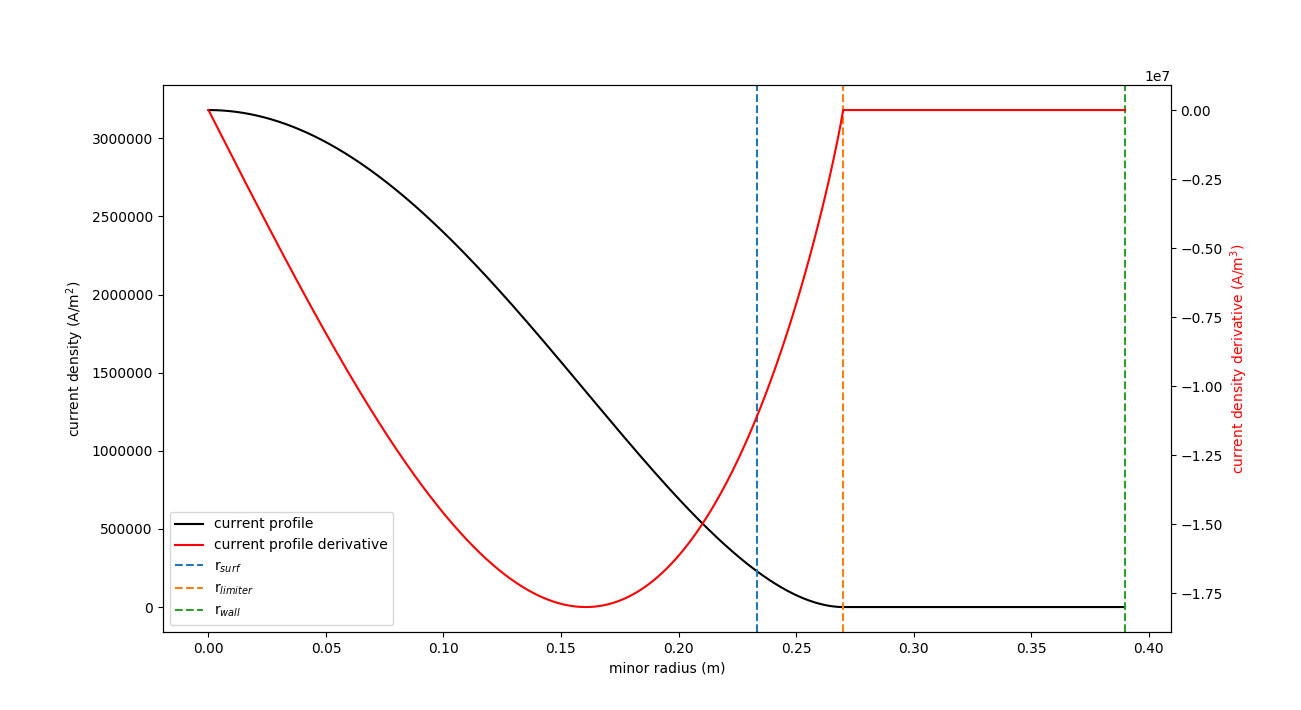
\includegraphics[width=15cm]{images/wessonCurrentProfile.png}
	\caption{Current profile and derivative
		\label{fig:schedule}}    
\end{figure}  

\noindent Possibly $q(0)$ and $q(a)$ could be adjusted to get slightly different current profiles.  


The q-profile is a little more difficult.  The 2003 paper made no mention other than constraining $q(0)$ and $q(a)$.  The 2014 paper suggested the cylindrical approximation

\begin{equation} \label{qCylindrical}
\begin{split}
q_{cyl}(r)=\frac{2(l+1)B_T}{\mu_0 j(0) R} \frac{(r/a)^2}{1-\left[ 1-(r/a)^2\right]^{l+1}}
\end{split} 
\end{equation} 

\noindent However, this equation is not valid for $r>a$, and I need $q(r)$ defined all the way to $r=b$.  

The paper also made mention to 

\begin{equation} \label{qDef}
\begin{split}
q(r)=\frac{2B_T}{\mu_0 \left<j(r)\right> R}
\end{split} 
\end{equation} 

\noindent where $\left<j(r)\right>$ is the average current density inside the radius $r$.  Because the system is in cylindrical coordinates, it's unclear if the average should be of $j(r)$ or $rj(r)$.  The average of $j(r)$ provides a q profile more similar to Eq.~\ref{qCylindrical}, but it places the resonant surface outside of the limiter.  

Instead, I'm presently using a quadratic q model, $q(r)=q(0)+cr^2$ until I figure out a better method.  This provides the following and the derivative of 1/q.  



\begin{figure}[htb]
	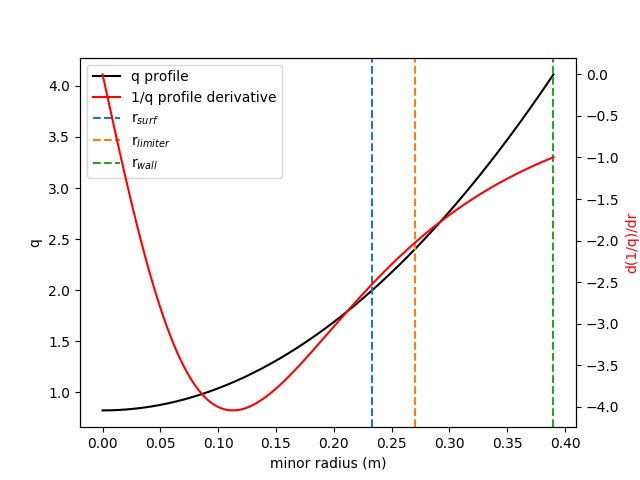
\includegraphics[width=15cm]{images/quadraticQProfile.png}
	\caption{Quadratic q profile and the derivative of 1/q.
		\label{fig:schedule}}    
\end{figure}  


%----------------------------------------------------------------------------------------
%	PROBLEM 2
%----------------------------------------------------------------------------------------


% %\bibliographystyle{plain}
% %\bibliography{bibFile.bib}
\bibliographystyle{apsrev}% ,isbn=false %[isbn=false]
\begin{thebibliography}{}

\bibitem{Chudnovskiy2003}
A. Chudnovskiy, Y. Gvozdkov, N. Ivanov, et. al.,
\emph{Nuclear Fusion}
{\bf 43} (2003). 

\bibitem{Ivanov2014}
N. V. Ivanov, A.M. Kakurin,
\emph{Physics of Plasmas}
{\bf 21}, 102502 (2014). 


\end{thebibliography}

%----------------------------------------------------------------------------------------

\end{document}

